%\documentclass[fleqn]{book}
\documentclass[11pt]{amsbook}

\usepackage[turkish]{babel}

%\usepackage{../HBSuerDemir}	% ------------------------
\usepackage{../Ceyhun}	% ------------------------
\usepackage{../amsTurkish}
\usepackage{tikz}
\newcommand*\circled[1]{\tikz[baseline=(char.base)]{
            \node[shape=circle,draw,inner sep=2pt] (char) {#1};}}

\begin{document}
% ++++++++++++++++++++++++++++++++++++++
\hPage{230}
% ++++++++++++++++++++++++++++++++++++++
\begin{proof}
gösterilsen ve $d_{i}$ (1$\leq i \leq$ 5)  $\circled{i}$ rengi ile boyanmış olsun (Şekil 4.5.2).

\begin{figure}[htb]
	\centering
	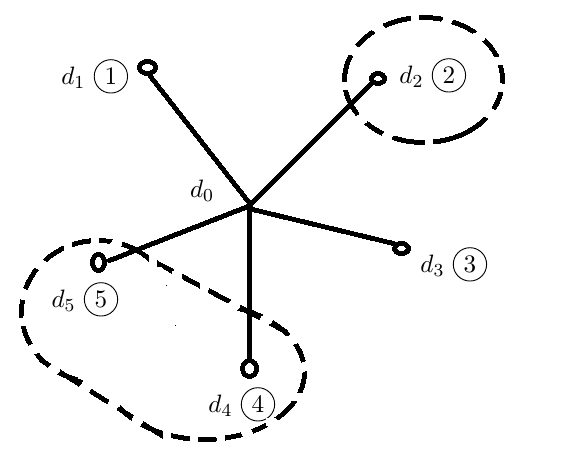
\includegraphics[width=0.45\textwidth]{images/ceyhun-230-fig01}
	\caption{5-boyanırlığın tanıtı.}
\end{figure}

$Ç_{1}$ çizgisinde, $\circled{1}$ ve $\circled{3}$ ile boyanmış düğümlerin irgittiği alçizgeyi $Ç_{2}$ ile gösterelim. $Ç_{2}$, genellikle parçalı bir çizge olacaktır. Eğer $d_{1}$ ve $d_{2}$ düğümleri, $Ç_{2}$ çizgesinin iki ayrı parçası içindeyse $d_{1}$ düğümünün bulunduğu parçadaki düğümlerin rengini değiştirebiliriz. Bu işlem sonucu, $d_{1}$ düğümüne bitişik düğümlerin boyanmasında  $\circled{1}$ kullanılmamış olacaktır. Öyleyse $d_{0}$ düğümünü  $\circled{1}$e boyayabiliriz ve $Ç(d,a)$ 5-boyanırdır.

Eğer $d_{1}$ ve $d_{2}$ düğümleri, $Ç_{2}$ çizgesinin aynı parçası içindeyse, $Ç_{2}$de yalnız $\circled{1}$ ve $\circled{3}$ ile boyanmış düğümleri içeren bir $Y_{13}$ yolu vardır.
\end{proof}
\end{document}